\documentclass[twocolumn]{IEEEtran}
\usepackage[utf8x]{inputenc}
\usepackage{amssymb,amsfonts}
\usepackage[tbtags]{amsmath}
\usepackage{graphicx}
\usepackage{cite}
\usepackage{slashbox}
\usepackage{pict2e}
\usepackage{float}
\usepackage[all]{xy}
\usepackage{graphics,graphicx,color,colortbl}
\usepackage{times}
\usepackage{subfigure}
\usepackage{wrapfig}
\usepackage{multicol}
\usepackage{cite}
\usepackage{url}
\usepackage[tbtags]{amsmath}
\usepackage{amsmath,amssymb,amsfonts,amsbsy}
\usepackage{bm}
\usepackage{algorithm}
\usepackage{algorithmic}
\usepackage[centerlast, small]{caption}
\usepackage[colorlinks=true, citecolor=blue, linkcolor=blue, urlcolor=blue,
breaklinks=true]{hyperref}

\begin{document}
\title{Respuesta en frecuencia (Resonancia)}
\author{José Fabio Lozano Ovalle Código: $222982$\\
	Wilson Orlando Macias Fuquen Código: $223101$\\
	David Ricardo Martínez Hernández Código: $261931$}
\maketitle
\markboth{Universidad Nacional de Colombia}{}
\floatname{algorithm}{Algoritmo}

\begin{abstract}
Se implementara un circuito $RLC$ serie que se encuentre en resonancia, teniendo en cuenta las condiciones de funcionamiento del generador de señales, se hallara la respuesta del circuito a la frecuencia midiendo valores experimentales de corriente y tensión para los elementos y finalmente se hallaran el ancho de banda y factor de calidad del circuito.
\end{abstract}

\begin{keywords}
Bobina, Condensador, Decibel, Energía, Frecuencia de Resonancia, Función de Transferencia, Ganancia, Resonancia.
\end{keywords}

\section{Objetivos}
\begin{itemize}
 \item Obtener una frecuencia de resonancia $\omega _0$ o $2*\pi f$, de acuerdo a los elementos utilizados en la práctica.
 \item Obtener la curva característica de un circuito $RLC$ en frecuencia, con un factor de calidad superior a $3$.
 \item Determinar el ancho de banda, la frecuencia de resonancia y el factor de calidad experimental del circuito $RLC$ serie.
\end{itemize}

\section{Introducción}
\noindent
El análisis de la respuesta en frecuencia es de gran importancia en el estudio de los fenómenos físicos, en este caso particular, los eléctricos, pues constituyen una base para comprender de una manera mejor conceptos como estabilidad o inestabilidad. También es de vital aplicación en el campo de las comunicaciones donde es necesario el diseño de dispositivos generadores y receptores, que puedan diferenciar entre determinados espectros frecuenciales. Es también utilizado en el diseño de sistemas de filtrado, sistemas de amplificación e innumerables aplicaciones. En resumen conocer el manejo de señales en el dominio frecuencia es una  herramienta matemática muy poderosa que nos ayuda a comprender mejor el estudio de las señales.

\section{Hipótesis}
\noindent
Se espera a que el voltaje se encuentre en fase con la corriente, debido a que las reactancias son iguales en magnitud, esto quiere decir que la reactancia total es cero y solo queda el valor resistivo. A demás se espera obtener un factor de calidad superior a $3$.\\
La reactancia del generador no debería influir en el comportamiento del circuito y el error obtenido debe ser pequeño.


\section{Materiales}
\begin{itemize}
 \item Bobina
 \item Condensador
 \item Generador de Señales
 \item Multímetro
 \item Osciloscopio
 \item Resistencias
\end{itemize}

\section{Análisis y Resultados}
\noindent
Para esta práctica se implementara un circuito $RLC$, para el cual se analiza la respuesta en frecuencia y se calcula la frecuencia de resonancia.
\begin{figure}[H]
	\centering
		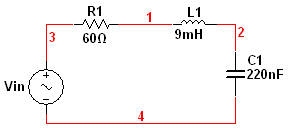
\includegraphics[scale=0.8]{circ1.PNG}
	\caption{Circuito RLC}
	\label{circ1}
\end{figure}
\noindent
Se tienen tres impedancias en serie las cuales son:
\begin{equation}
Z_R=R
\label{ecuR}
\end{equation}
\begin{equation}
Z_L=j \omega_0 L
\label{ecuL}
\end{equation}
\begin{equation}
Z_C =  \frac{1}{j\omega_0 C}
\label{ecuC}
\end{equation}
\noindent
Donde la impedancia total esta dada por
\begin{equation}
Z= R + j(\omega_0 L - \frac{1}{\omega_0 C})
\label{ecu101}
\end{equation}
\noindent
Para que $Z$ sea puramente real se debe cumplir que
\begin{equation}
\omega_0 L - \frac{1}{\omega_0 C}=0
\label{ecu102}
\end{equation}
\noindent
Despejando $\omega_0$ se tiene que la frecuencia de resonancia es
\begin{equation}
\omega_0=\sqrt{\frac{1}{LC}}
\label{ecu103}
\end{equation}
\noindent
Para el circuito de la Fig. \ref{circ1} se calcula una frecuencia de resonancia de
\begin{equation}
\omega_0=\sqrt{\frac{1}{(9mH)(0.22\mu F)}}=22473.328 Rad/seg
\label{ecu104}
\end{equation}
\noindent
\begin{equation}
f_0=\frac{\omega_0}{2 \pi}=\frac{22473.328Rad/seg}{2 \pi}=3576.741 Hz
\label{ecu104}
\end{equation}
\noindent
Con un factor de calidad
\begin{equation}
Q=\frac{L\omega_0}{R}=3.371
\label{ecu104}
\end{equation}
\noindent
Además  se tiene un ancho de banda
\begin{equation}
B=\frac{R}{L}=\frac{60\Omega}{9mH}=6666.67 Rad/seg=1061.0329 Hz
\label{ecu104}
\end{equation}
\noindent
Se realizo el montaje de la Fig. \ref{circ1}, con una frecuencia $f_{0} = 3.576\ KHz$ $\omega = 2\pi f_{0} = 3.579\ KHz * 2 \pi$, una resistencia de un valor de $60.2\ \Omega$. Los valores obtenidos se encuentran en la siguiente tabla
\begin{table}[H]
	\centering
\begin{tabular}[c]{|c|c|} \hline
$V_{DC}$ & $8 \ V$ \\ \hline
$V_{RMS}$ & $4.04 \ V_{rms}$ \\ \hline
$V_{pico}$ & $6.4 \ V_{pico}$ \\ \hline
$V_{C}$ & $7.40 \ V_{rms}$ \\ \hline
$V_{R}$ & $2.136 \ V_{rms}$ \\ \hline
$V_{L}$ & $5.765 \ V_{rms}$ \\ \hline
$V_{fuente}$ & $2.445 \ V_{rms}$ \\ \hline
\end{tabular}
	\caption{Valores obtenidos en la práctica a la frecuencia $f_0$}
	\label{tab1}
\end{table}
\begin{figure}[H]
 \centering
    \subfigure[Salida de resonancia para la frecuencia $f_0$]{\label{fig1a}
      \fbox{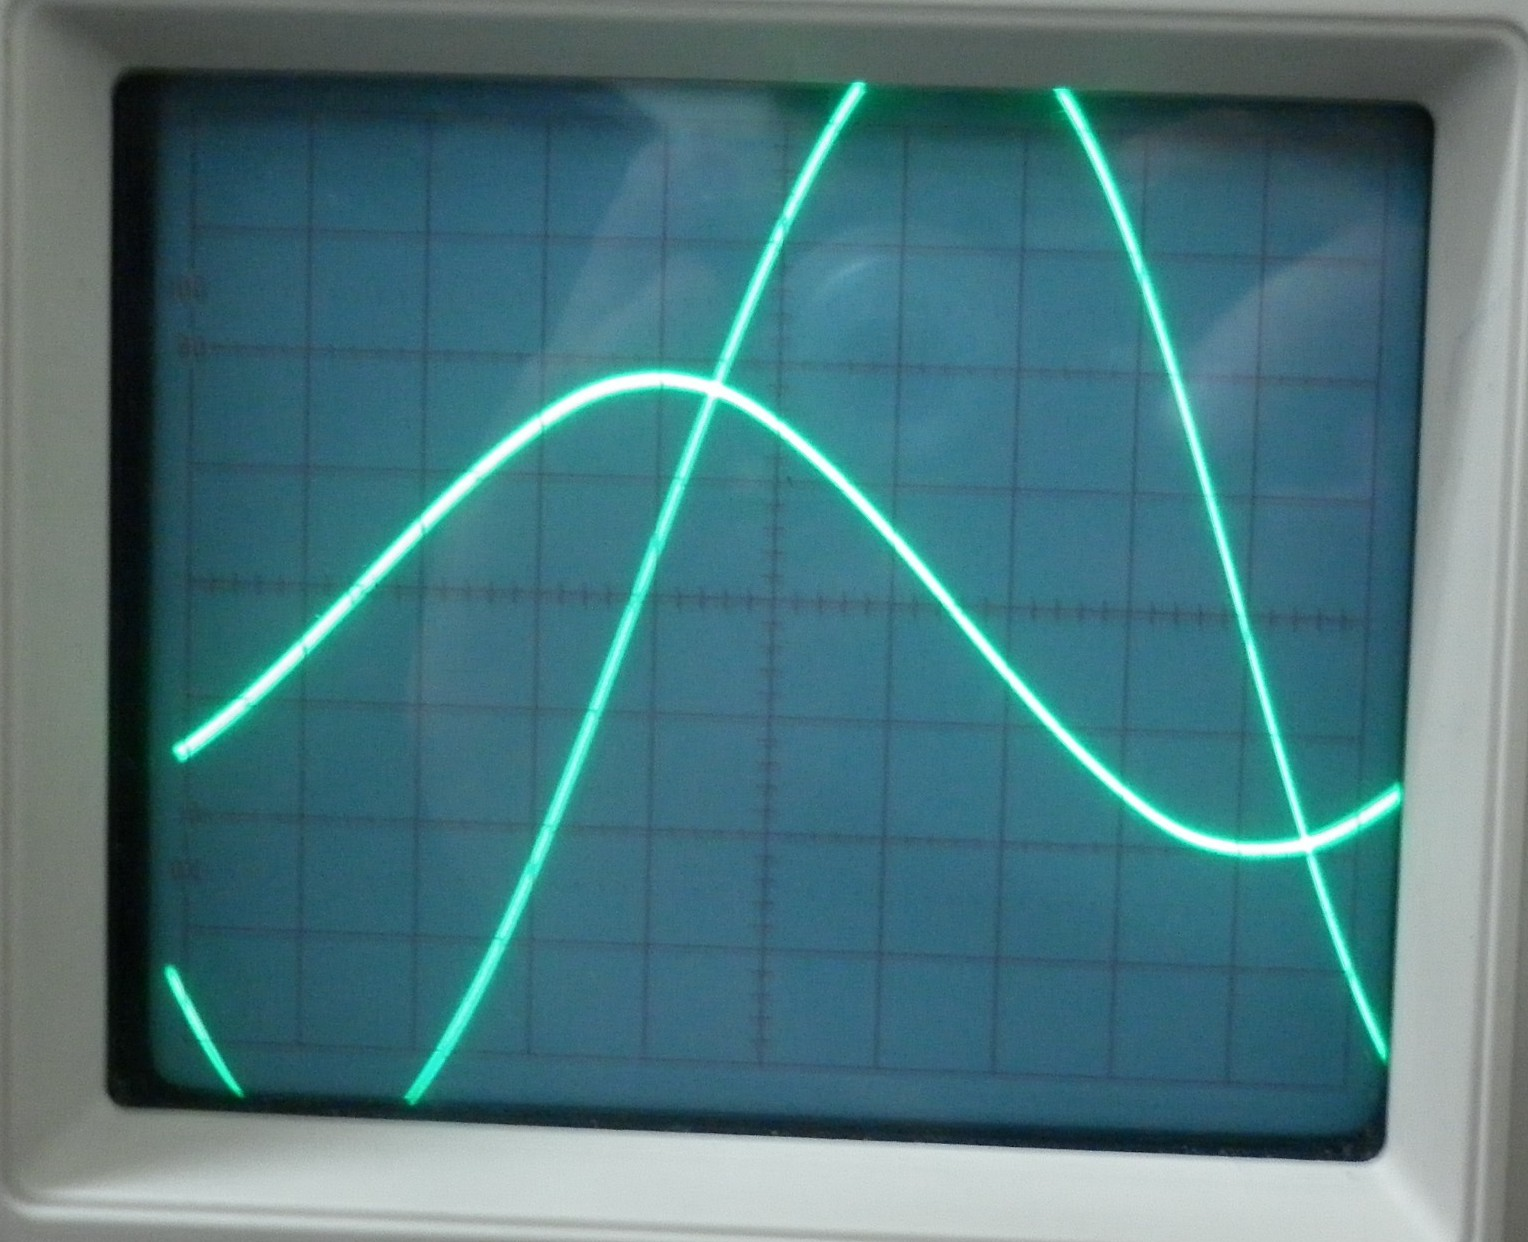
\includegraphics[scale=0.13]{360.png}}}
  \hspace{2cm}
    \subfigure[Salida de resonancia para la frecuencia $f_0$]{\label{fig1b}
      \fbox{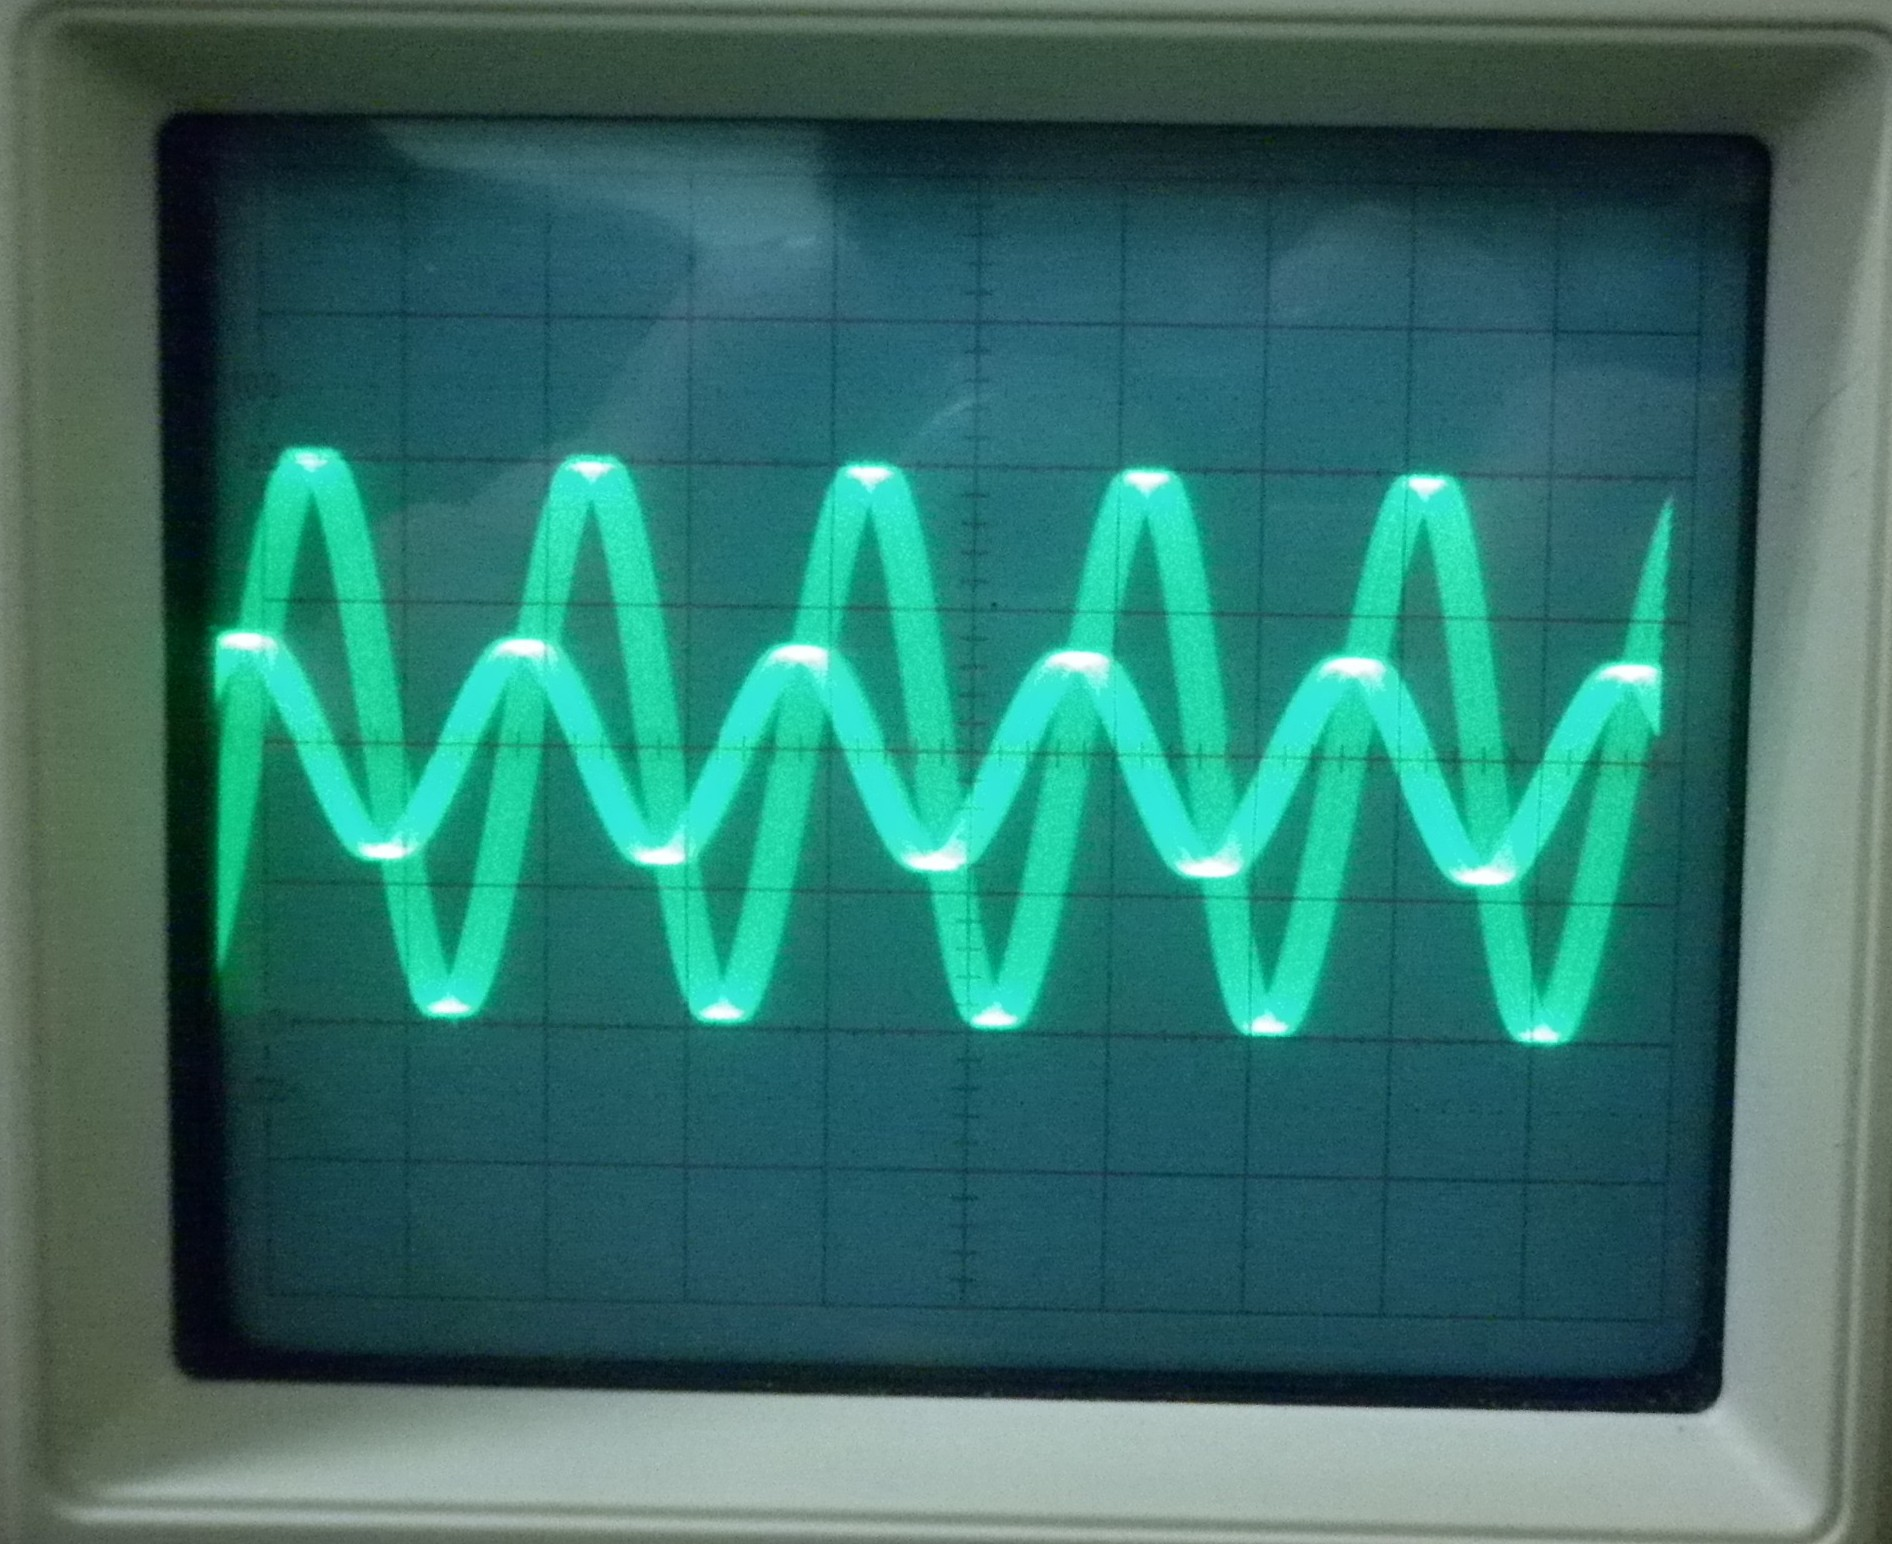
\includegraphics[scale=0.1]{365.png}}}
  \caption{Salida de resonancia para la frecuencia $f_0$}
    \label{fig1}
\end{figure}
\noindent
La salida de la simulación se muestra a continuación Fig. \ref{teo1}
\begin{figure}[H]
	\centering
		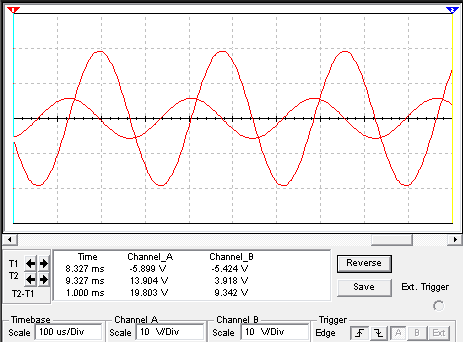
\includegraphics[scale=0.5]{sim.png}
	\caption{Salida de resonancia teórica para la frecuencia $f_0$}
	\label{teo1}
\end{figure}
\noindent
La TAB \ref{tabteo1} de valores obtenidos 
\begin{table}[H]
	\centering
\begin{tabular}[c]{|c|c|} \hline
$V_{RMS}$ & $4.04 \ V_{rms}$ \\ \hline
$V_{C}$ & $13.605 \ V_{rms}$ \\ \hline
$V_{R}$ & $4.04 \ V_{rms}$ \\ \hline
$V_{L}$ & $13.632 \ V_{rms}$ \\ \hline
\end{tabular}
	\caption{Valores obtenidos en las simulaciones a la frecuencia $f_0$}
	\label{tabteo1}
\end{table}
\noindent
Se cambio la frecuencia a $f_m = 6.574\ KHz$, los valores de los condensadores, de las bobinas y de las resistencias constantes, dando como resultado
\begin{table}[H]
	\centering
\begin{tabular}[c]{|c|c|} \hline
$V_{DC}$ & $8 \ V$ \\ \hline
$V_{RMS}$ & $4.04 \ V_{rms}$ \\ \hline
$V_{pico}$ & $6.4 \ V_{pico}$ \\ \hline
$V_{C}$ & $0.819 \ V_{rms}$ \\ \hline
$V_{R}$ & $0.688 \ V_{rms}$ \\ \hline
$V_{L}$ & $3.324 \ V_{rms}$ \\ \hline
$V_{fuente}$ & $2.445 \ V_{rms}$ \\ \hline
\end{tabular}
	\caption{Valores obtenidos en la práctica a la frecuencia $f_m$}
	\label{tab2}
\end{table}
\begin{figure}[H]
	\centering
		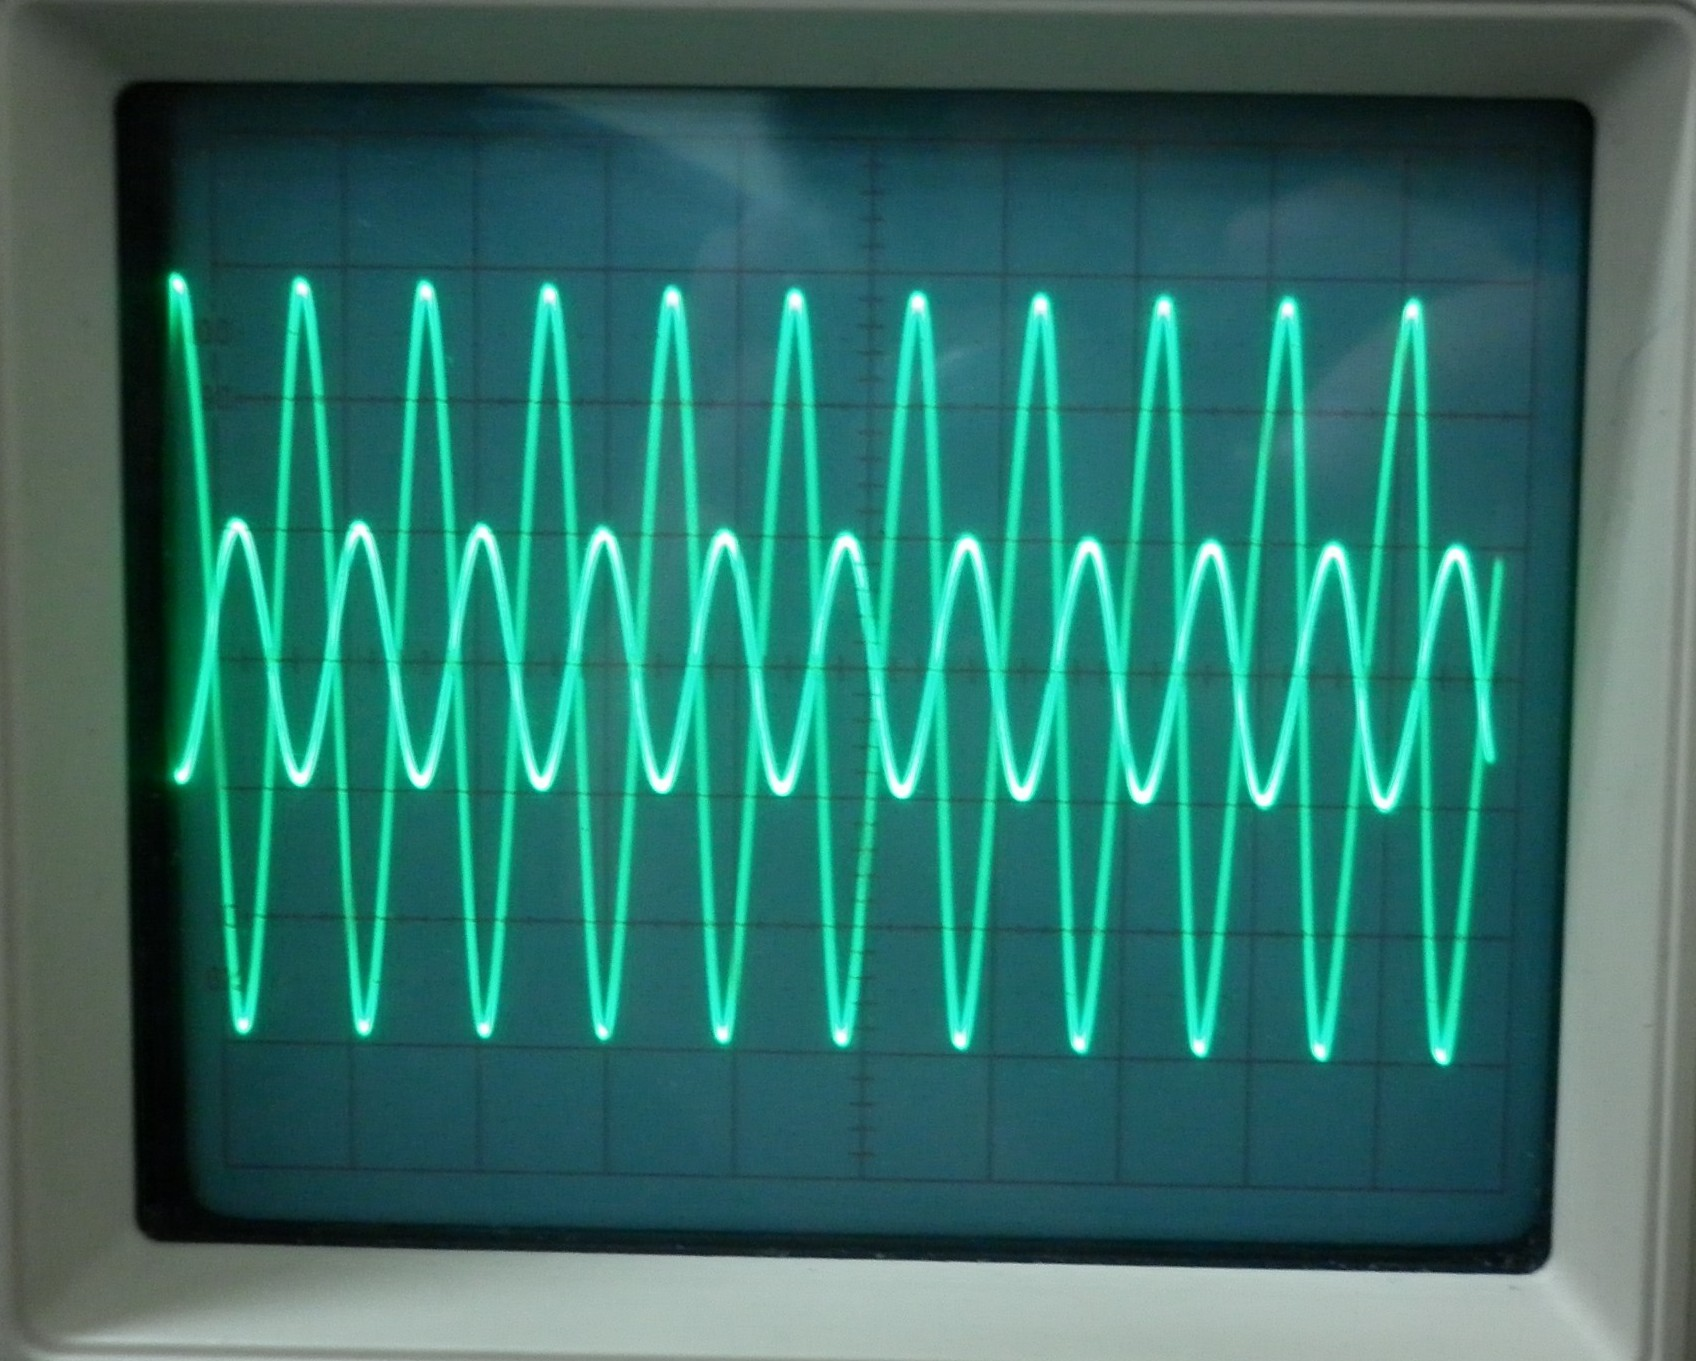
\includegraphics[scale=0.1]{366.png}
	\caption{Salida de resonancia para la frecuencia $f_m$}
	\label{fig2}
\end{figure}
\noindent
La salida de la simulación se muestra a continuación Fig. \ref{teo2}
\begin{figure}[H]
	\centering
		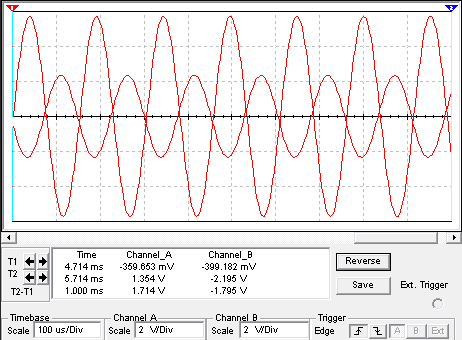
\includegraphics[scale=0.5]{sim1.png}
	\caption{Salida de resonancia teórica para la frecuencia $f_m$}
	\label{teo2}
\end{figure}
\noindent
La TAB \ref{tabteo2} de valores obtenidos 
\begin{table}[H]
	\centering
\begin{tabular}[c]{|c|c|} \hline
$V_{RMS}$ & $4.04 \ V_{rms}$ \\ \hline
$V_{C}$ & $1.651 \ V_{rms}$ \\ \hline
$V_{R}$ & $901.05 \ mV_{rms}$ \\ \hline
$V_{L}$ & $5.589 \ V_{rms}$ \\ \hline
\end{tabular}
	\caption{Valores obtenidos en las simulaciones a la frecuencia $f_m$}
	\label{tabteo2}
\end{table}
\noindent
Se cambio la frecuencia a $f_u = 10.19\ KHz$, los valores de los condensadores, de las bobinas y de las resistencias constantes, dando como resultado
\begin{table}[H]
	\centering
\begin{tabular}[c]{|c|c|} \hline
$V_{DC}$ & $8 \ V$ \\ \hline
$V_{RMS}$ & $4.04 \ V_{rms}$ \\ \hline
$V_{pico}$ & $6.4 \ V_{pico}$ \\ \hline
$V_{C}$ & $2.49 \ nV_{rms}$ \\ \hline
$V_{R}$ & $0.358 \ V_{rms}$ \\ \hline
$V_{L}$ & $2.267 \ V_{rms}$ \\ \hline
$V_{fuente}$ & $2.445 \ V_{rms}$ \\ \hline
\end{tabular}
	\caption{Valores obtenidos en la práctica a la frecuencia $f_u$}
	\label{tab3}
\end{table}
\begin{figure}[H]
	\centering
		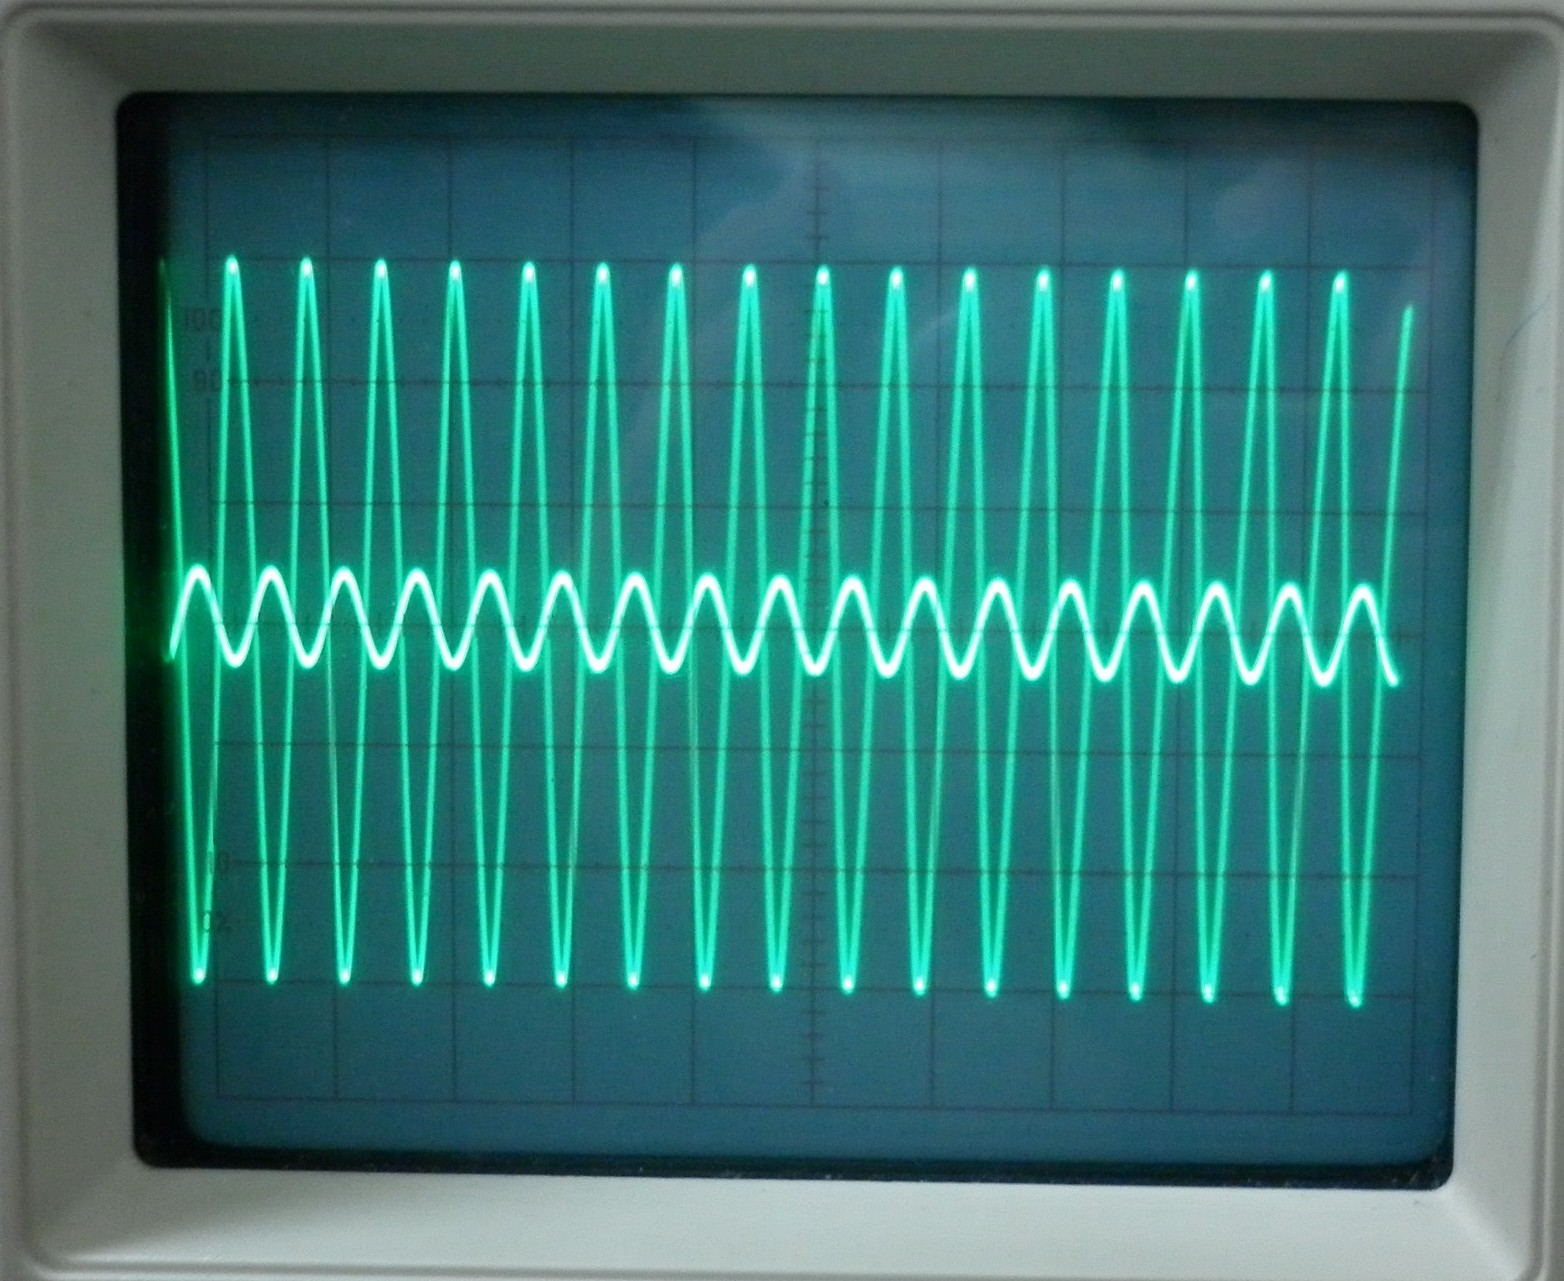
\includegraphics[scale=0.1]{367.png}
	\caption{Salida de resonancia para la frecuencia $f_u$}
	\label{fig3}
\end{figure}
\noindent
La salida de la simulación se muestra a continuación Fig. \ref{teo3}
\begin{figure}[H]
	\centering
		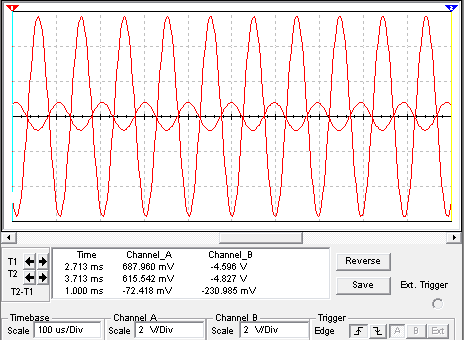
\includegraphics[scale=0.5]{sim2.png}
	\caption{Salida de resonancia teórica para la frecuencia $f_u$}
	\label{teo3}
\end{figure}
\noindent
La TAB \ref{tabteo3} de valores obtenidos 
\begin{table}[H]
	\centering
\begin{tabular}[c]{|c|c|} \hline
$V_{RMS}$ & $4.04 \ V_{rms}$ \\ \hline
$V_{C}$ & $328.913 \ mV_{rms}$ \\ \hline
$V_{R}$ & $480.358 \ mV_{rms}$ \\ \hline
$V_{L}$ & $4.587 \ V_{rms}$ \\ \hline
\end{tabular}
	\caption{Valores obtenidos en las simulaciones a la frecuencia $f_u$}
	\label{tabteo3}
\end{table}
\noindent
Se cambio la frecuencia a $f_d = 200.3\ Hz$, los valores de los condensadores, de las bobinas y de las resistencias constantes, dando como resultado
\begin{table}[H]
	\centering
\begin{tabular}[c]{|c|c|} \hline
$V_{DC}$ & $8 \ V$ \\ \hline
$V_{RMS}$ & $4.04 \ V_{rms}$ \\ \hline
$V_{pico}$ & $6.4 \ V_{pico}$ \\ \hline
$V_{C}$ & $4.237 \ V_{rms}$ \\ \hline
$V_{R}$ & $82.2 \ mV_{rms}$ \\ \hline
$V_{L}$ & $16.7 \ mV_{rms}$ \\ \hline
$V_{fuente}$ & $2.445 \ V_{rms}$ \\ \hline
\end{tabular}
	\caption{Valores obtenidos en la práctica a la frecuencia $f_d$}
	\label{tab4}
\end{table}
\begin{figure}[H]
	\centering
		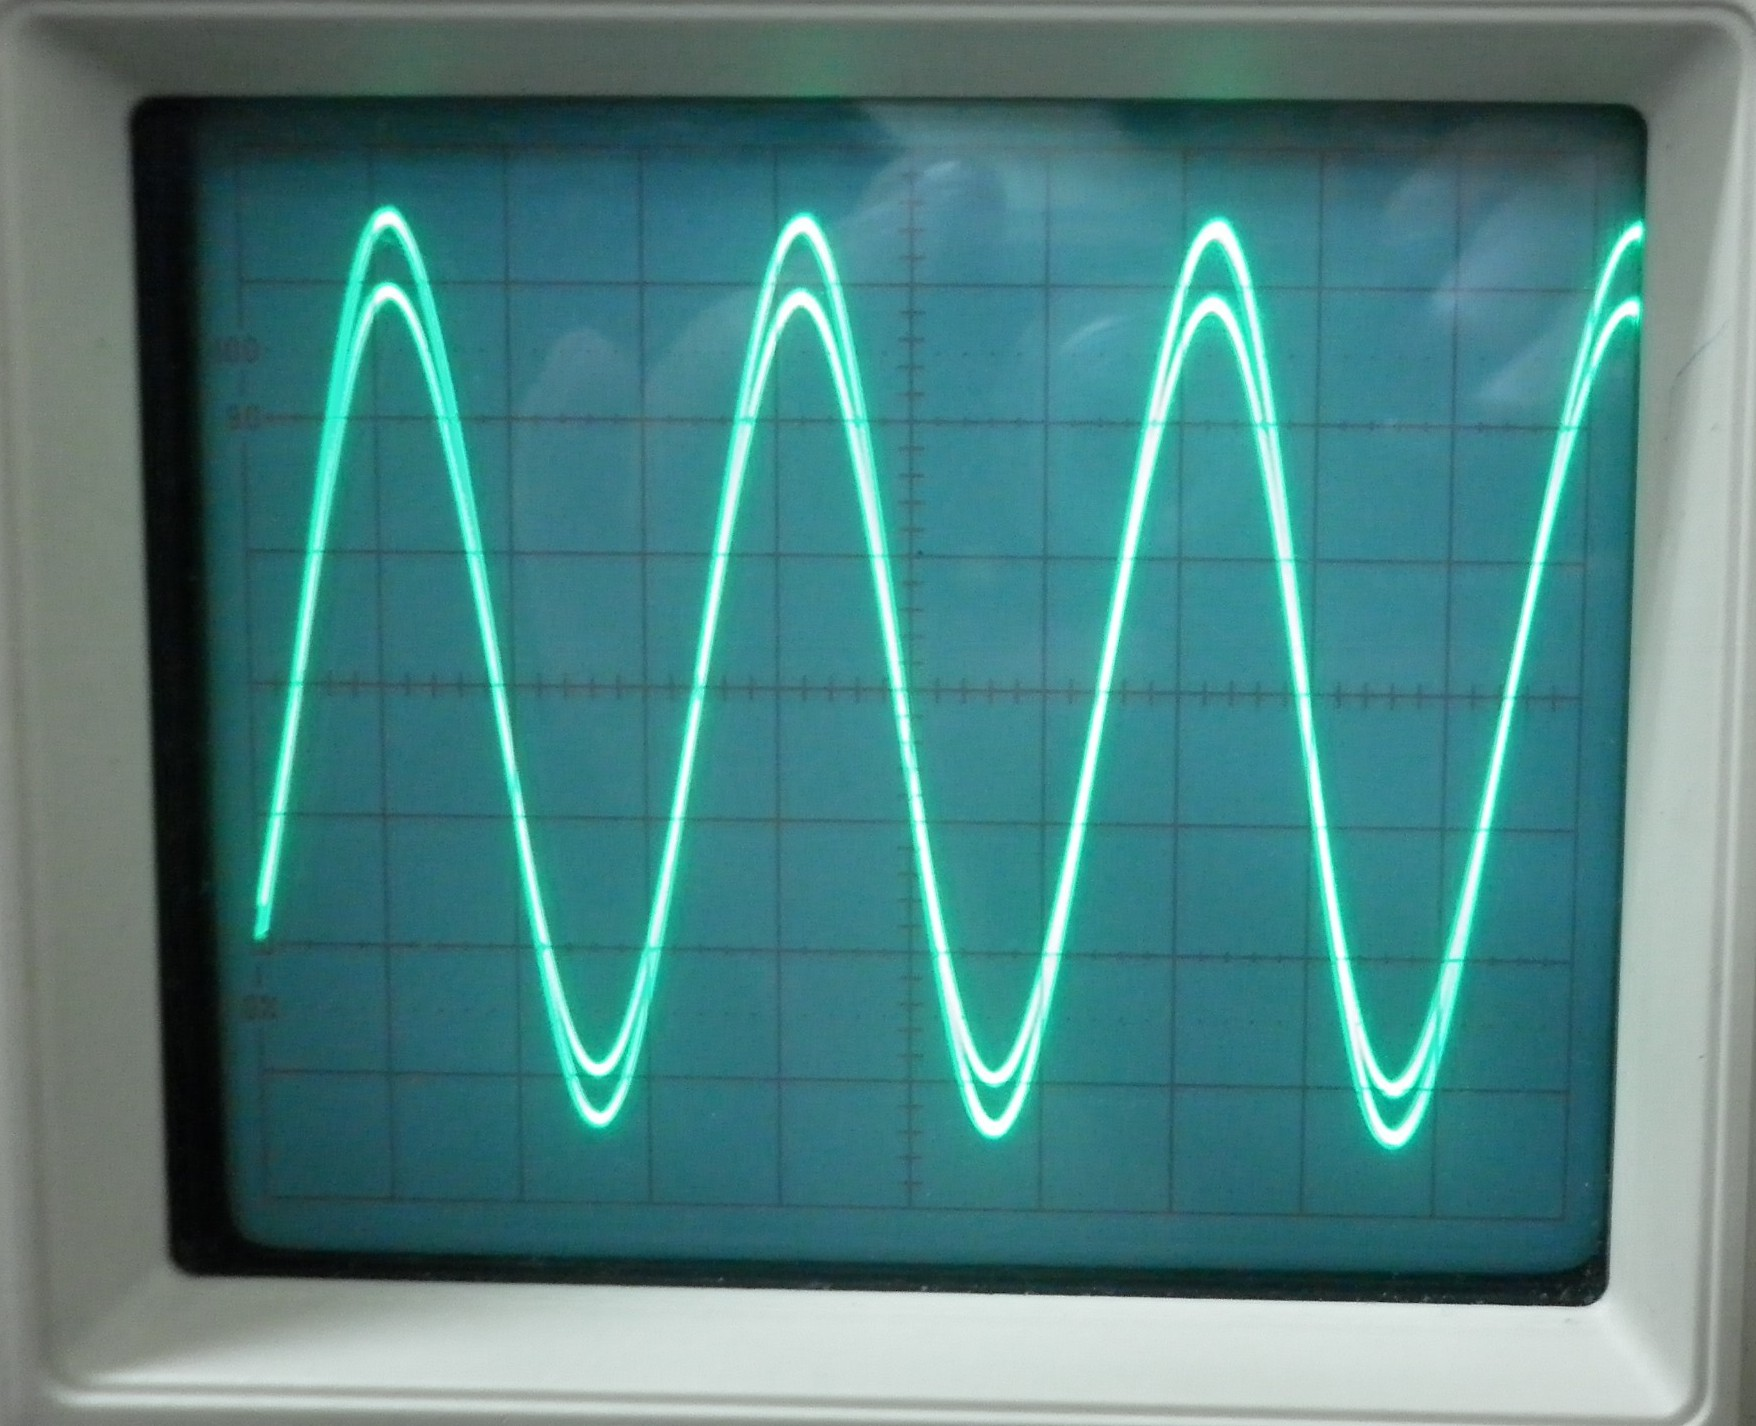
\includegraphics[scale=0.1]{368.png}
	\caption{Salida de resonancia para la frecuencia $f_d$}
	\label{fig4}
\end{figure}
La salida de la simulación se muestra a continuación Fig. \ref{teo4}
\begin{figure}[H]
	\centering
		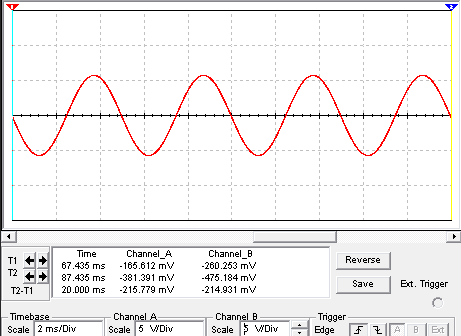
\includegraphics[scale=0.5]{sim3.png}
	\caption{Salida de resonancia teórica para la frecuencia $f_d$}
	\label{teo4}
\end{figure}
\noindent
La TAB \ref{tabteo4} de valores obtenidos 
\begin{table}[H]
	\centering
\begin{tabular}[c]{|c|c|} \hline
$V_{RMS}$ & $4.04 \ V_{rms}$ \\ \hline
$V_{C}$ & $4.052 \ V_{rms}$ \\ \hline
$V_{R}$ & $67.294 \ mV_{rms}$ \\ \hline
$V_{L}$ & $12.708 \ mV_{rms}$ \\ \hline
\end{tabular}
	\caption{Valores obtenidos en las simulaciones a la frecuencia $f_d$}
	\label{tabteo4}
\end{table}
\noindent
\begin{figure}[H]
	\centering
		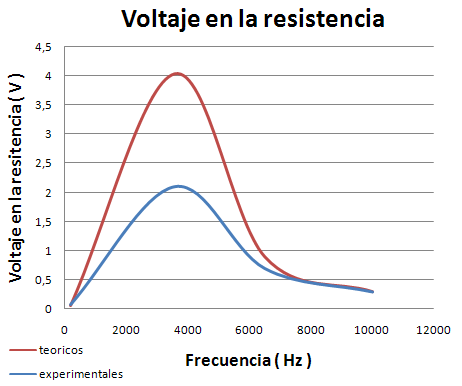
\includegraphics[scale=0.6]{vrvsfr.png}
	\caption{Gráfico comparativo de frecuencia con respecto al voltaje en $R$}
	\label{teo5}
\end{figure}
\noindent
Para diferentes frecuencias se midió el valor de tensión sobre los tres elementos y se encontró
que en la frecuencia de resonancia teórica de $3.576\ KHz$ se presenta el comportamiento
esperado, es decir se obtiene el máximo voltaje sobre la resistencia. Los voltajes de la bobina
y condensador son parecidos. El voltaje en la resistencia es más pequeño que el esperado
teóricamente debido a la impedancia interna del generador de señales, esto hace que caiga de
$4.04\ V$ teóricos a $2.136\ V$ experimentales.\\
En baja frecuencia el comportamiento de las tensiones teóricas y experimentales fue muy
parecido, pero en alta frecuencia el valor de tensión en el condensador fue más elevado
que el teórico. Esto sucede porque en el capacitor aparece una componente resistiva no
despreciable en alta frecuencia, y deja de comportarse como un capacitor puro.\\
Se presentaron inconvenientes al momento de calibrar las mediciones con el osciloscopio, esto
no se pudo explicar, y nos genero grandes dificultades al momento de realizar las mediciones,
tiempo después el osciloscopio permitió realizar las mediciones pero creemos que esto pudo
incidir en la efectividad de los datos tomados con el osciloscopio.

\section{Preguntas}
\begin{enumerate}
 \item ¿En que consiste el fenómeno de resonancia?\\
Es la condición que existe en un sistema físico cuando una función forzada de amplitud fija produce una respuesta de amplitud máxima, en el caso eléctrico se presenta este fenómeno cuando la impedancia de la red es puramente resistiva o mas exactamente cuando la reactancia se anula, como consecuencia tenemos que si una red esta en resonancia la tensión y la corriente en las terminales de entrada de la red están en fase.

 \item ¿Qué es Factor de calidad, ancho de banda y Frecuencia de resonancia ($F_o$)?\\
La frecuencia de resonancia es el valor que se necesita en un circuito para que se presente el fenómeno de resonancia, esto se debe a que en los elementos como capacitores e inductores las reactancias dependen directamente de la frecuencia.
\begin{equation}
 {F_0} = \frac{1}{{2\pi \sqrt {LC} }}
\label{ecu50}
\end{equation}
\noindent
El ancho de banda es el intervalo de frecuencias que comprende los valores de potencia media, también se puede calcular con la corriente del circuito, ya que sabemos que la corriente máxima se da en la frecuencia de resonancia y los valores de frecuencia que corresponden al $0.707$ de la corriente máxima son los mismos de la potencia media.
\begin{figure}[H]
	\centering
		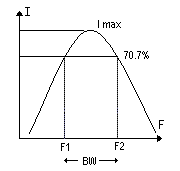
\includegraphics[scale=0.7]{figura1.png}
	\caption{Ancho de banda en función de la corriente}
	\label{figura1}
\end{figure}
\begin{equation}
 {B_\omega } = {F_2} - {F_1}
\label{ecu51}
\end{equation}
\noindent
El factor de calidad es la cantidad que se puede almacenar en un circuito, en comparación con la energía que se pierde durante un periodo completo de la respuesta. En términos de la frecuencia el factor de calidad $Q$ para un circuito $RLC$ serie es:
\begin{equation}
 Q = \frac{{2\pi {F_0}}}{{{B_\omega }}} = \frac{{2\pi {F_0}L}}{R}
\label{ecu52}
\end{equation}

 \item ¿Que sucede con la frecuencia de resonancia, el factor de calidad, y el ancho de banda
al variar independientemente $R$ o $L$ o $C$?\\
Para la frecuencia de resonancia si variamos R no se altera pero si cambiaos $L$ o $C$ habrá un cambio en esta. El factor de calidad depende de todos los valores porque un en $C$ cambiaría la frecuencia de resonancia vemos que el factor de calidad también depende de $L$ y $R$. El ancho de banda depende solamente de $R$ directamente y de $L$ de forma inversa, es decir aumenta cuando $R$ aumenta y disminuye cuando $L$ aumenta.

 \item ¿Cual es valor de la tensión $V_L + V_C$ en la práctica? ¿Concuerda con la teoría? Explique.\\
Dicho valor para la frecuencia $f_0$, su valor práctico es de  $13.165\ V$ y el teórico es de $17.645\ V$, para la frecuencia $f_m$, su valor práctico es de $4.143\ V$ y el teórico es de $7.24\ V$, para la frecuencia $f_u$, su valor práctico es de $2.267\ V$ y el teórico es de $4.915\ V$,  para la frecuencia $f_d$, su valor práctico es de $4.253\ V$ y el teórico es de $4.064\ V$.La diferencia entre los valores medidos y los obtenidos teóricamente es debido al no conocer los valores reales de todos los elementos, se tuvieron problemas con el osciloscopio, el generador de señales y los demás elementos utilizados en la práctica. Se sumaron las magnitudes de los voltajes.\\
El valor teórico de $VL+VC$ es cero pero en la practica a la frecuencia de resonancia teórica de
$3.576\ KHz$ es de $1.7\ V_{rms}$, esto se debe a que el circuito experimental presenta una frecuencia
de resonancia diferente al teórico.

 \item ¿Que impacto tiene el generador de señales en la respuesta del sistema?\\
Como la Impedancia del generador es diferente de cero, también es susceptible de cambiar respecto a la frecuencia, a frecuencias muy grandes la componente inductiva  de la impedancia del generador será muy grande y frecuencias muy pequeñas la componente capacitiva es la que será considerable, entonces para algunos valores será grande la contribución en  determinada reactancia del generador a nuestro circuito.
\end{enumerate}

\section{Conclusiones}
\begin{itemize}
 \item El comportamiento de la tensión en la resistencia experimentalmente es muy similar al teórico, lo que nos permite afirmar que la frecuencia de resonancia experimental del circuito es muy cercana a la teórica. No fue posible calcular el valor exacto de la frecuencia de resonancia experimental por problemas de medida con el osciloscopio.
 \item Los valores de tensión teóricos y experimentales pueden cambiar en condiciones extremas de funcionamiento, por ejemplo el capacitor deja de comportarse de manera ideal en alta frecuencia, ya que aparece una componente resistiva no despreciable.
 \item Caracterizando el voltaje de la resistencia en función de la frecuencia es posible determinar la frecuencia de resonancia del circuito, ya que su máximo mostrara el punto en que la potencia activa del circuito es máxima y la potencia reactiva es cero.
\end{itemize}

\bibliographystyle{ieeetran}
\begin{thebibliography}{99}
\bibitem{sadiku} Alexander, Charles K. \&  Sadiku, Matthew N.O.
{\em ```Fundamentals of Electric Circuits"'}.
McGRAW-HILL, ISE Editions, 1999.

\bibitem{dorf} Dorf  \& Svoboda.
{\em ```Circuitos Eléctricos"'}.
Alfaomega, Sexta Edición, 2006.

\bibitem{hayt} Hayt, William H. Jr., Kemmerly, Jack E. \& Durbin, Steven M.
{\em ```Análisis de circuitos en ingeniería"'}.
McGRAW-HILL, Séptima Edición, 2007.

\bibitem{nahvi} Nahvi, Mahmood \& Edminister, Joseph A.
{\em ```Theory and Problems of Electric Circuits"'}.
McGRAW-HILL, Fourth Edition, 2003.

\end{thebibliography}
\end{document}